\section{التحكم التكيفي المعتمد على العزم المحسوب (\LR{Adaptive Computed Torque Control})}
\label{sec:actc_control}

\subsection*{1. مبدأ الخوارزمية}
تدمج هذه الخوارزمية بين تقنية الإلغاء الخطي للديناميكية (\LR{Feedback Linearization}) وبين آلية تكيفية مستمرة لتحديث معلمات النظام المجهولة (مثل كتلة الحمل وعزوم القصور الذاتي) في الزمن الفعلي. يتم استبدال الثوابت الفيزيائية المجهولة بمعلمات مُقَدَّرَة تتحدث قيمتها بناءً على خطأ التتبع، مما يوفر أداءً ناعماً ومستقراً دون الحاجة لإشارات التبديل القاسية.

\subsection*{2. الشكل العام لقانون التحكم ومبدأ الانحدار}
تعتمد الخوارزمية على خاصية خطية المعلمات (\LR{Linearity in Parameters})، حيث يمكن فصل النموذج الديناميكي إلى مصفوفة انحدار (\LR{Regressor} $Y$) تحوي المتغيرات الحركية المعروفة، وشعاع معلمات ($\Theta$) يحوي الثوابت المجهولة. 

لتطبيق الخوارزمية بشكل عملي ومستقل لكل مفصل، يُكتب قانون التحكم التكيفي للمفصل $(i)$ بالصيغة القياسية التالية:
\begin{equation}
\tau_i = \hat{\theta}_i^T Y_i - K_{s,i} s_i
\label{eq:adaptive_general_i}
\end{equation}
حيث $\hat{\theta}_i$ هو شعاع المعلمات المُقَدَّرَة للمفصل، و $Y_i$ شعاع الانحدار الخاص به، و $s_i$ هو سطح الانزلاق، و $K_{s,i}$ ربح تحكم موجب لضمان تقارب الخطأ.

\subsection*{3. تفكيك النموذج وتعريف المعلمات المُقَدَّرَة}
بتفصيل المعادلة (\ref{eq:adaptive_general_i}) بناءً على القوى الفيزيائية المؤثرة على المفصل (عطالة، احتكاك، جاذبية)، يأخذ قانون التحكم شكله التفصيلي المطبق على المحركات كما يلي:
\begin{equation}
\tau_i = \hat{\theta}_{M,i} (M_e(q)\ddot{q}_r)_i + \hat{\theta}_{V,i} (K_v \dot{q})_i + \hat{\theta}_{G,i} G_i(q) + \hat{\theta}_{0,i} - K_{s,i} s_i
\label{eq:adaptive_detailed_i}
\end{equation}

حيث تم تخصيص معامل مُقَدَّر منفصل لكل مركب ديناميكي:
\begin{itemize}
    \item $\hat{\theta}_{M,i}$: المُعامل التكيفي المُقَدَّر لتعويض تغيرات عزم القصور الذاتي الكلي (والذي يتأثر بشدة بتغير كتلة الحمل $m_L$).
    \item $\hat{\theta}_{V,i}$: المُعامل المُقَدَّر لتعويض قوى الاحتكاك اللزج والقوى المرتبطة بالسرعة.
    \item $\hat{\theta}_{G,i}$: المُعامل المُقَدَّر لتعويض عزوم الجاذبية الأرضية.
    \item $\hat{\theta}_{0,i}$: المُعامل المُقَدَّر لتعويض الاحتكاك السكوني (\LR{Coulomb Friction}) والاضطرابات الثابتة المجهولة.
\end{itemize}

\subsection*{4. تعريف الأخطاء وقانون التحديث (\LR{Adaptation Law})}
يتم تعريف سطح الانزلاق للمفصل $(i)$ بالاعتماد على خطأ التتبع الموضعي $e_i = q_i - q_{ref,i}$ كالتالي:
\begin{equation}
s_i = \dot{e}_i + \lambda_i e_i
\end{equation}
حيث $\lambda_i$ ثابت إيجابي يحدد ميل السطح. ولتحديث المعلمات المُقَدَّرَة $\hat{\theta}_i$ لحظياً وبشكل يضمن استقرار النظام وفق نظرية ليابونوف، يتم تطبيق قانون التحديث التفاضلي المدعوم بتعديل سيغما (\LR{$\sigma$-modification}) لمنع انحراف القيم:
\begin{equation}
\dot{\hat{\theta}}_i = \Gamma_i Y_i^T s_i - \Gamma_i \sigma_i \hat{\theta}_i
\end{equation}
حيث $\Gamma_i$ مصفوفة أرباح التعلم اللحظي، و $\sigma_i$ عامل تخميد إيجابي صغير.
\subsection*{5. استجابة النظام عند قيم مختلفة للحمل ($m_L$)}
تم اختبار خوارزمية (\LR{ACTC}) لمحاكاة تتبع المسارات المرجعية ($\theta_{1ref} = \theta_{2ref} = 90^\circ$ و $d_{3ref} = 0.2 \text{ m}$) مع تغيير ظروف التحميل للتحقق من قدرة الخوارزمية على التكيف الذاتي:


 \begin{figure}[H]
     \centering
     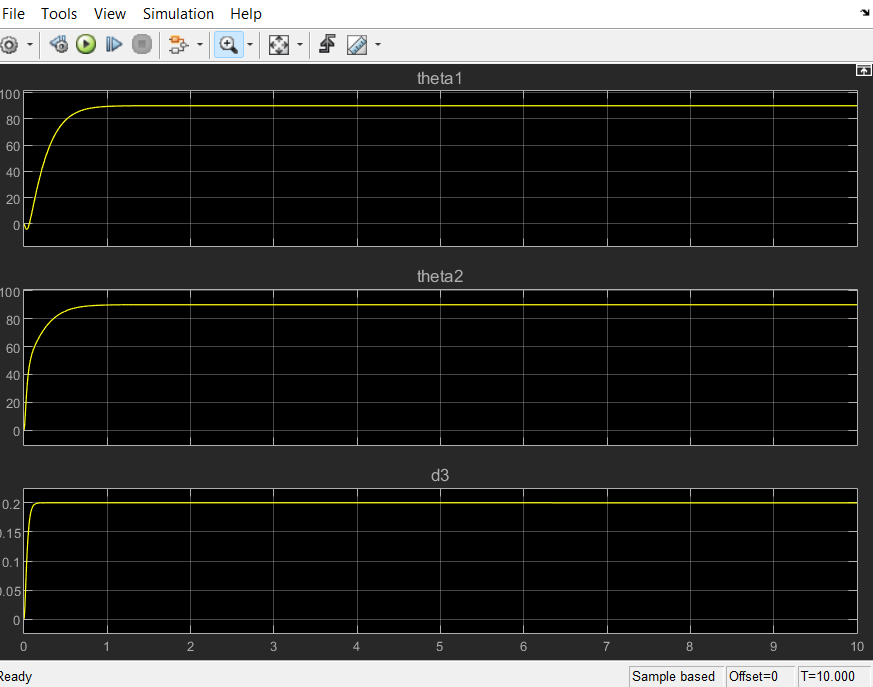
\includegraphics[width=0.8\textwidth]{resources/images/ACTC_res_m0.png}
     \caption{\centering{استجابة متحكم \LR{ACTC} وتتبع المسار بدون حمل ($m_L = 0 \text{ kg}$)}}
     \label{fig:actc_m0}
 \end{figure}

 \begin{figure}[H]
     \centering
     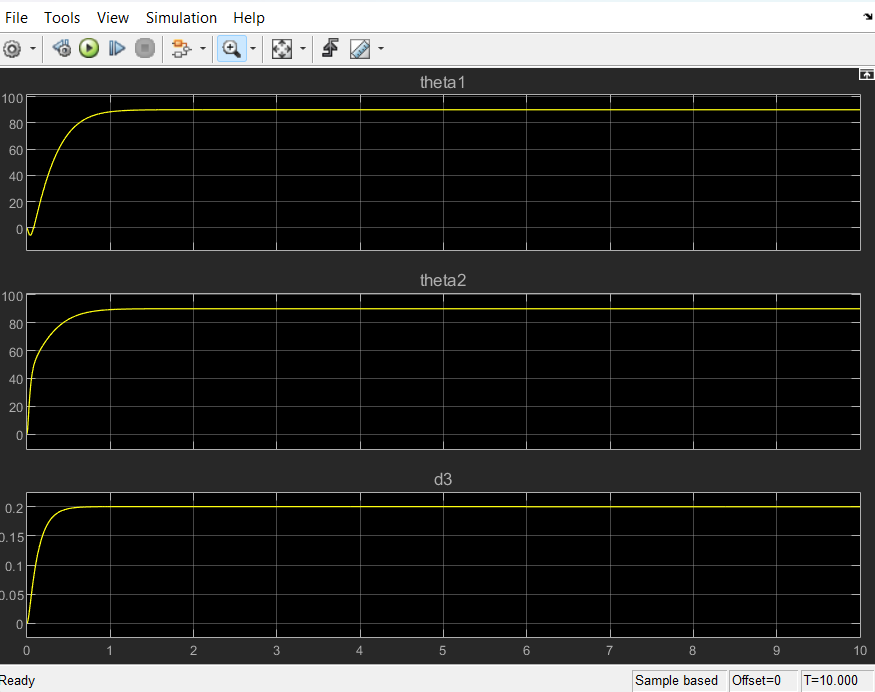
\includegraphics[width=0.8\textwidth]{resources/images/ACTC_res_m10.png}
     \caption{\centering{استجابة متحكم \LR{ACTC} وتحديث المعلمات لحظياً عند إضافة حمل ($m_L = 10 \text{ kg}$)}}
     \label{fig:actc_m10}
 \end{figure}

يُلاحظ من المنحنيات ظهور انحراف أولي سالب (\LR{Initial Undershoot}) لفترة وجيزة جداً في استجابة المفصل الأول ($\theta_1$) قبل انطلاقه نحو القيمة المرجعية. هذا الانحراف يعكس الطبيعة الفيزيائية الدقيقة للمحاكاة والتداخل الديناميكي (\LR{Dynamic Coupling}) بين المفاصل؛ فالتسارع الابتدائي العنيف للمفصل الثاني لتتبع المسار يولد عزم رد فعل يؤثر عكسياً على المفصل الأول، وسرعان ما تقوم خوارزمية (\LR{ACTC}) بتدارك هذا الاضطراب اللحظي وتصحيح المسار بقوة ونعومة.

بشكل عام، تظهر النتائج تفوقاً ديناميكياً وهندسياً واضحاً للمتحكم التكيفي. في حالة اللاحمل ($m_L = 0$)، استجاب النظام بسرعة فائقة محققاً زمن استقرار (\LR{Settling Time}) يقارب ($0.1 \text{ s}$). أما عند إضافة الحمل الأقصى المفاجئ ($10 \text{ kg}$)، فبدلاً من الانهيار كما في (\LR{PID}) أو استهلاك طاقة تبديل قاسية كما في (\LR{SMC})، قامت الآلية التكيفية بتقدير الزيادة اللحظية في القصور الذاتي وتحديث المعامل $\hat{\theta}_{M,3}$ داخلياً، ليتمكن النظام من استعادة استقراره التام خلال زمن قياسي لم يتجاوز ($0.5 \text{ s}$). نتج عن ذلك تتبع مسار عالي الدقة، وإشارات تحكم ناعمة خالية من ظاهرة الاهتزاز (\LR{Chattering})، مما يجعله الحل الأمثل صناعياً.